\section{Aula 6.5 - Interferencia intersimbólica}

Nessa aula veremos o conceito de interferência intersimbólica e como quantizar o erro trazido pela mesma.

\subsection{O que é interferência intersimbólica?}

Quando um sinal é transmitido depois de ser modulado é esperado que  forma do pulso enviado seja contida no intervalo de envio de um símbolo, mas o meio de transmissão não é ideal
e consequentemente ruído no canal ou tensão residual fará o pulso perdurar por um "tempinho a mais" e invadir o espaço de outro pulso se isso ocorrer e os pulsos não forem devidamente
espaçados por exemplo 101 na codificação RZ-UniPolar seria um exemplo  de codificação fácil de diminuir esse problema visto que um zero é ausência de pulso e consequentmente sequência de bits
com 0's no meio evitam que ocorra interferência de pulsos e consequentemente o bit recebido é detectado incorretamente.
\\

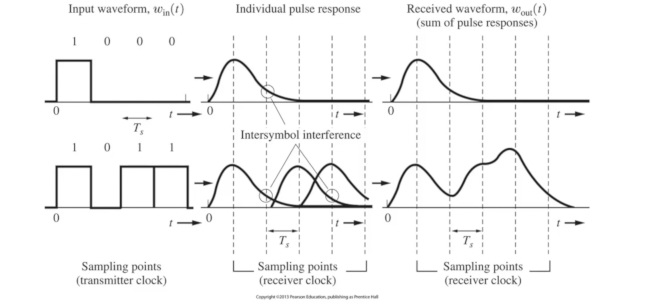
\includegraphics[width=0.8\textwidth]{../assets/iis.png}\cite{dc}

\subsection{Fourier ao resgate}


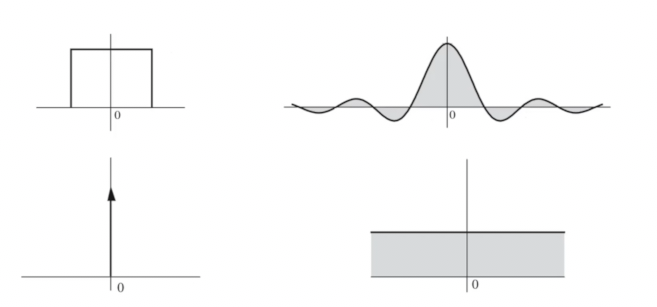
\includegraphics[width=0.8\textwidth]{../assets/fourier.png}\cite{dc}

Nessa imagem o lado esquerdo é a função expressa no domínio do tempo e no lado direito é a função no domínio da frequência, obtida através da transformada de Fourier.

Note que a função no superior esquerdo é essencialmente um pulso recebido da saída do sistema de comunicação, mas uma análise detalhada, função superior direita, é impossível
que o canal transmita sem distorção.

e se inverter o raciocínio e e pensar na função sinc como sendo o sinal no tempo o problema ocorre visto que é agora no tempo que ocorerrá a IIS, interferência intersimbólica.

\subsection{A solução de Harry Nyquist}

O engenheiro Nyquist, pesquisador na área de teoria da informação, notou que seria possível garantir detecção de IIS se a largura de banda fosse igual a metade da taxa de transmissão de bits.
então a conclusão prática é que o espectro do sinal enviado é uma função porta e é possível detetar o símbolo enviado examinando o pico da função sinc que a cada $h(t-kT)$ isto é ler o sinal recebido
no meio de um período vai ocasionar em IIS, mas ler no momento exato elimina o problema.

O problema é que esse filtro é teórico e impossível de ser constrúido na prática, mas existe o filtro cosseno levantado que pode ser utilizado como alternativa.
\\\\
\textbf{OBS:} uma função que satisfaz esses critérios de Nyquist é pertencente a classe de Nyquist na literatura.

\subsection{Aproximando o ideal}


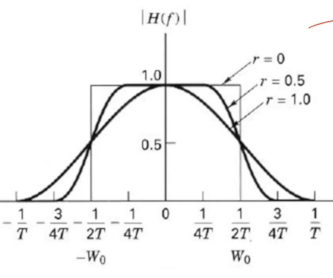
\includegraphics[width=0.4\textwidth]{../assets/cos.png}\cite{dc}

o parâmetro \textbf{r} visto na figura  é chamado de fator de decaimento e é responsável por dizer o quão rápido é a aproximação de tal filtro do filtro ideal de Nyquist.
a equação que computa r é a seguinte:
\begin{equation}
	r = \frac{W - W_o}{W_o}
\end{equation}

Se r é 1 então o filtro tem o dobro da banda do filtro de nyquist e consequentemente a maior redução de IIS possível, mas note o custo, aumento na largura de banda, enquanto que se
r < 0 então a IIS só tende a aumentar visto que as componentes espectrais ficam mais difíceis de "caber" na largura de banda do meio.


